\documentclass{standalone}
\usepackage{tikz}
\usetikzlibrary{positioning, arrows.meta, shapes.geometric}

\begin{document}

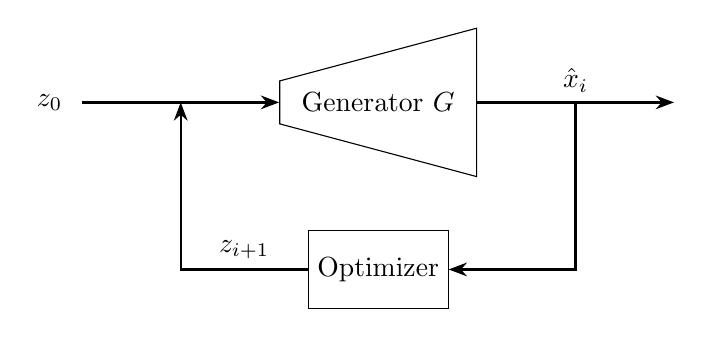
\begin{tikzpicture}[
    latent/.style={circle, draw, minimum size=1cm, node distance=2cm},
    trapezoid/.style={trapezium, shape border rotate=90, trapezium angle=75, draw, minimum height=2.5cm, minimum width=1cm, node distance=2cm},
    block/.style={rectangle, draw, minimum size=1cm, node distance=2cm},
    arrow/.style={-Stealth, thick},
]

% Nodes
\node (A) {};
\node[trapezoid, right=2.5cm of A] (generator) {Generator $G$};
\node[right=2.5cm of generator] (B) {};
\node[block, below=1cm of generator] (optimizer) {Optimizer};

% Arrows
\draw[arrow] (A) node[left] {$z_0$} -- (generator.west) node[midway, above] (middle_left) {};
\draw[arrow] (generator.east) -- (B) node[midway, above] (middle_right) {$\hat{x}_i$};
\draw[arrow] (middle_right) |- (optimizer.east);
\draw[arrow] (optimizer.west) -| (middle_left) node[near start, above] {$z_{i + 1}$};

\end{tikzpicture}

\end{document}
